% !TEX ROOT = ../ersti.tex
%\section*{Beratung und Informationen zum Lehramt}
\newpage\subsection{\Large Beratung und Informationen zum Lehramt}%FIXME
\begin{itemize}
\item Rechtsverbindliche Auskünfte zu Pädagogik, Fächerkombinationen und
      den Staatsprüfungen gibt es beim Landeslehrerprüfungsamt. \newline
      \textbf{Landeslehrerprüfungsamt (LPA) Baden-Württemberg,
           Außenstelle Karlsruhe},
      Kreuzstr.~11, 76133~Karlsruhe; \newline
Tel.~07\,21/92\,64\,50\,0~(Leiter), 07\,21/92\,64\,50\,2~(Herr Ehret) \newline
      \url{http://www.uni-heidelberg.de/studium/imstudium/pruef_lehramt.html} \newline
      jeden 1. Dienstag im Monat, 14:30 bis 17:00 Uhr,
      \textbf{\gls{ZUV}, Seminarstraße 2, Raum 149}


\item \textbf{Zentrum für Lehrerbildung (ZLB)} und \textbf{Zentrale Studienberatung\,/\,Career Service (ZSB)} \newline
      kurze Auskünfte: Service Portal, \gls{ZUV}, Seminarstraße 2, im Erdgeschoss (am Haupteingang links)
      Öffnungszeiten: Siehe online\footnote{\url{http://www.uni-heidelberg.de/studium/kontakt/}} \newline
      Termin für ein Beratungsgespräch: \\ Tel. 0\,62\,21\,/\,54\,-\,54\,54

      \url{http://zlb.uni-hd.de}\\
      \url{http://studienberatung.uni-hd.de}

\item Die „Verordnung des Kultusministeriums über die Erste Staatsprüfung für das
Lehramt an Gymnasien (Gymnasiallehrerprüfungsordnung I)“, kurz „Lehramts-PO“, gibt es im ZLB oder
      im Internet verlinkt auf:

      \url{http://www.uni-heidelberg.de/studium/download/index.html#stud}


\item Der AK Lehramt des StuRa\footnote{\url{http://www.stura.uni-heidelberg.de}}
      gibt gemeinsam mit der  GEW-Studierendengruppe ein Lehramtsinfo heraus: \newline AK
      Lehramt des StuRa/GEW"-Studierendengruppe, c/o~StuRa-Büro, Alber-Ueberle-Straße~3-5; Tel:~0\,62\,21/54\,24\,56

      \url{http://www.stura.uni-heidelberg.de/arbeitskreise/ak-lehramt.html}



\item Noch mehr Infos gibt es im Café mit Lehramtsberatung im
      Erziehungswissenschaftliches Seminar, Do 14 bis 18 Uhr,
      anschließend von 18 bis 20 Uhr Vorträge, Filme und Infos für
      Lehramtsstudierende.
\end{itemize}


%~ \begin{figure}[h]
%~ \centering{
    %~ 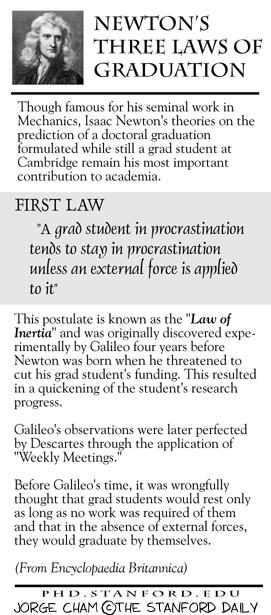
\includegraphics[width=3.5cm]{bilder/newton_1.png}
    %~ \hspace{0.55cm}
    %~ 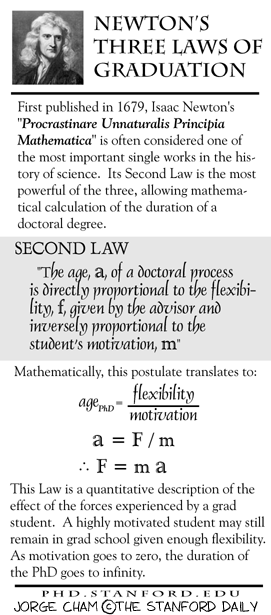
\includegraphics[width=3.5cm]{bilder/newton_2.png}
    %~ \hspace{0.55cm}
    %~ 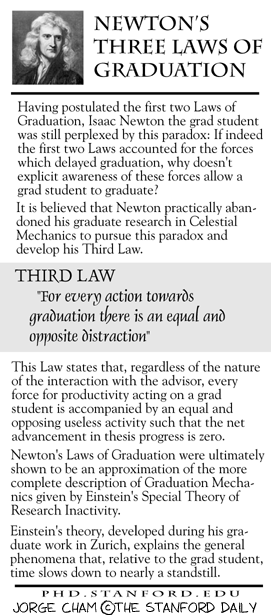
\includegraphics[width=3.5cm]{bilder/newton_3.png}
%~ }
%~ \end{figure}
